\section{Ablation}\label{sec:ablation}

\subsection{What each element contributes}

Table~\ref{tab:abl} gives the ratio $\rho$ of the 95th percentiles and the efficiency ratio $\eta$ of each variant of the method, as the median over seeds 1 to 3 with the range of $\rho$; Fig.~\ref{fig:ablation} shows the ratios. Every variant is scored on the acceptance ensemble against the phase-fixed WGS hologram of its own seed, and differs from the method in one element.
The rows are read in groups.

\emph{Design samples.} Minimizing the nominal cost with the same solver, budget, level and start (one design point at the origin) does not lower the spread: $\rho=\ablNominalMed$ (\ablNominalMin{} to \ablNominalMax) at $\eta=\ablNominalEff$, so the gain is not the work of the extra iterations, and a hologram pushed toward a level of $0.9$ of its own efficiency without the aberration terms is worse than the starting one. Random draws held fixed during the descent
recover part of the gain, and the gain grows with their number: $\rho$ is \ablRandFourMed{} for 4 draws, \ablRandEightMed{} for 8, \ablRandSixteenMed{} for 16 and \ablRandThirtyTwoMed{} for 32. The 16 sigma points reach \ablDefaultMed{}, above the range of 16 random draws (up to \ablRandSixteenMax) and above the median of 32. Resampling 8 random draws at every step with Adam gives \ablAdamMed{} (\ablAdamMin{} to \ablAdamMax) at the highest
efficiency of the group, $\eta=\ablAdamEff$. H4 holds: for the same number of design samples the deterministic set gives the larger ratio, and the deterministic set also costs the fewest evaluations of the cost for the ratio it reaches.

\emph{Modes in the design.} A design that covers part of the modes of the ensemble does not protect against the rest. With defocus only $\rho$ is \ablModesDefocusMed, with Noll 4 to 6 \ablModesToSixMed, with Noll 4 to 8 \ablModesToEightMed, and a design on Noll 9 to 11, which are not the modes that dominate the ensemble spread, gives \ablModesHighMed; only the full set of eight reaches \ablDefaultMed. An incomplete design is worse than the baseline on the full ensemble; the measurement does not isolate the mechanism, and the result is the reason the designed modes must cover the modes of the residual.

\emph{Design amplitude.} The design amplitude has a sharp optimum at the amplitude of the ensemble, $0.02$ waves per mode: $\rho$ is \ablPriorAMed{} at 0.005, \ablPriorBMed{} at 0.01, \ablDefaultMed{} at 0.02, \ablPriorDMed{} at 0.03 and \ablPriorEMed{} at 0.04. The target level was held at \parLevel{} in all of these, and the level is tied to the amplitude by the Strehl ratio (Section~\ref{sec:results}), so a change of the amplitude alone moves the design off its best level; the
ablation varies one element at a time and does not map the pair.

\subsection{Level and iterations}

Figure~\ref{fig:level} plots the trade-off of the level. A level of $0.80$ lowers the efficiency to \ablLevelAEff{} of the baseline and the ratio to \ablLevelAMed; levels of $0.85$, $0.90$, $0.937$, $0.95$ and $1.00$ give \ablLevelBMed, \ablDefaultMed, \ablLevelDMed, \ablLevelEMed{} and \ablLevelFMed{} at efficiency ratios of \ablLevelBEff, \ablDefaultEff, \ablLevelDEff, \ablLevelEEff{} and \ablLevelFEff. The ratio is highest at the level of
$0.90$, near the Strehl ratio of the ensemble (\strehlExp), and falls on both sides; higher levels return the efficiency to or above that of the baseline (the efficiency ratio is above one from $0.937$ on) and give up part of the gain, so the level is the dial between efficiency and robustness. A user who needs to keep the full efficiency of phase-fixed WGS can take $\ell=0.937$, which keeps $\eta\ge1$ at a ratio of \ablLevelDMed.

\begin{table}[t]
\centering\small
\caption{Ablation on seeds 1 to 3 against the acceptance ensemble: ratio $\rho$ of the 95th percentiles of phase-fixed WGS and of each variant (median and range over seeds) and efficiency ratio $\eta$ (median). The variants differ from the method in one element: the design samples, the modes in the design, the design amplitude, the target level and the number of conjugate-gradient iterations.}
\label{tab:abl}
\begin{tabular}{@{}l r l r@{}}
\toprule
Variant & $\rho$ (median) & range & $\eta$\\
\midrule
\emph{Design samples} & & & \\
\quad sigma points, 16 deterministic draws (B4) & 1.43 & 1.42 to 1.57 & 0.982 \\
\quad nominal cost only, same CG (one point) & 0.62 & 0.56 to 0.71 & 0.891 \\
\quad 4 fixed random draws, same CG & 1.00 & 0.98 to 1.12 & 0.952 \\
\quad 8 fixed random draws, same CG & 1.20 & 1.12 to 1.21 & 0.972 \\
\quad 16 fixed random draws, same CG & 1.33 & 1.26 to 1.36 & 0.974 \\
\quad 32 fixed random draws, same CG & 1.39 & 1.33 to 1.44 & 0.980 \\
\quad resampled draws (8 per step), Adam & 1.24 & 1.16 to 1.28 & 0.988 \\
\midrule
\emph{Modes in the design} & & & \\
\quad defocus only (Noll 4) & 0.75 & 0.59 to 0.82 & 0.901 \\
\quad Noll 4 to 6 & 0.92 & 0.70 to 0.92 & 0.924 \\
\quad Noll 4 to 8 & 1.17 & 1.13 to 1.17 & 0.952 \\
\quad Noll 9 to 11 (not the dominant modes) & 0.89 & 0.75 to 0.94 & 0.924 \\
\quad Noll 4 to 11 (B4) & 1.43 & 1.42 to 1.57 & 0.982 \\
\midrule
\emph{Design amplitude} & & & \\
\quad design amplitude 0.005 waves per mode & 0.65 & 0.60 to 0.75 & 0.898 \\
\quad design amplitude 0.01 waves per mode & 0.84 & 0.83 to 0.87 & 0.916 \\
\quad design amplitude 0.02 waves per mode (B4) & 1.43 & 1.42 to 1.57 & 0.982 \\
\quad design amplitude 0.03 waves per mode & 1.13 & 1.07 to 1.23 & 1.012 \\
\quad design amplitude 0.04 waves per mode & 0.90 & 0.90 to 0.98 & 1.016 \\
\midrule
\emph{Target level} & & & \\
\quad target level 0.80 & 0.71 & 0.53 to 0.78 & 0.849 \\
\quad target level 0.85 & 1.25 & 1.04 to 1.29 & 0.929 \\
\quad target level 0.90 (B4) & 1.43 & 1.42 to 1.57 & 0.982 \\
\quad target level 0.937 & 1.27 & 1.24 to 1.33 & 1.006 \\
\quad target level 0.95 & 1.19 & 1.18 to 1.26 & 1.009 \\
\quad target level 1.00 & 1.06 & 1.04 to 1.14 & 1.014 \\
\midrule
\emph{Iterations} & & & \\
\quad 5 CG iterations & 1.30 & 1.28 to 1.36 & 0.981 \\
\quad 10 CG iterations & 1.33 & 1.27 to 1.37 & 0.978 \\
\quad 20 CG iterations & 1.40 & 1.39 to 1.53 & 0.981 \\
\quad 40 CG iterations (B4) & 1.43 & 1.42 to 1.57 & 0.982 \\
\quad 80 CG iterations & 1.44 & 1.42 to 1.56 & 0.984
\\
\bottomrule
\end{tabular}
\end{table}

\begin{figure}[t]
\centering
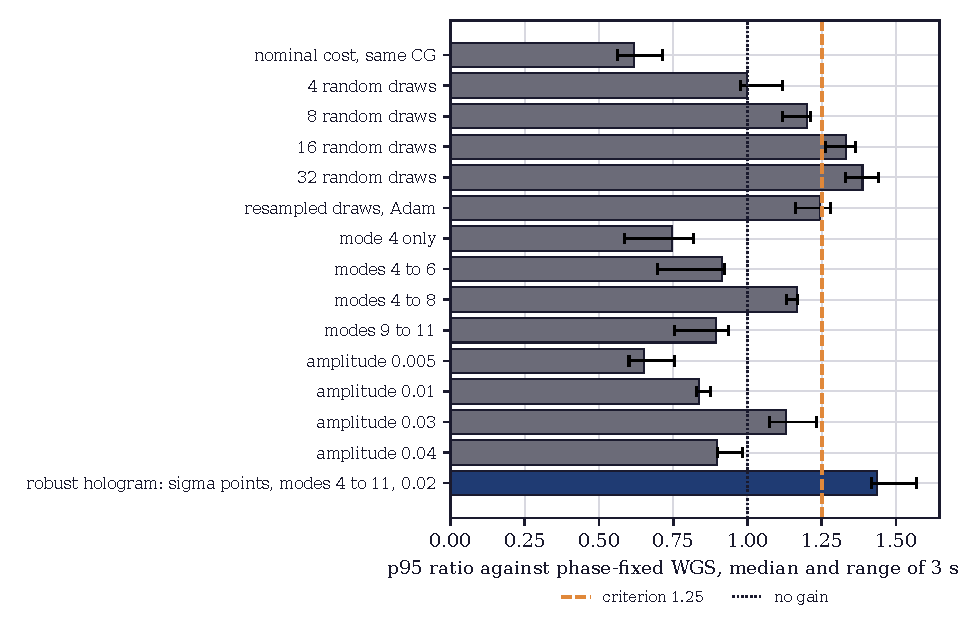
\includegraphics[width=0.8\textwidth]{fig-ablation.pdf}
\caption{Ratio of the 95th percentiles against phase-fixed WGS for each variant of the design samples, the modes and the design amplitude, median and range over three seeds, with the full method as the dark bar; the dashed line is the criterion of 1.25 and the dotted line marks no gain.}
\label{fig:ablation}
\end{figure}

\begin{figure}[t]
\centering
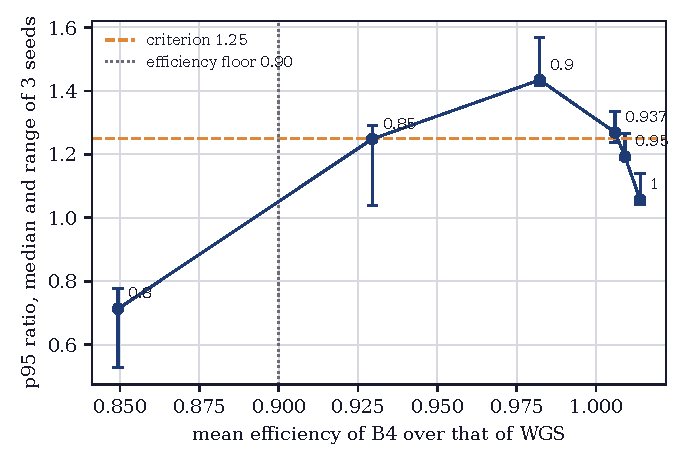
\includegraphics[width=0.62\textwidth]{fig-level.pdf}
\caption{Trade-off of the target level: ratio of the 95th percentiles against the efficiency ratio for target levels from 0.80 to 1.00 (labels), median and range of three seeds; the dashed line is the criterion of 1.25 and the dotted line the efficiency floor of 0.90.}
\label{fig:level}
\end{figure}

The iterations (Fig.~\ref{fig:conv}) matter little beyond the first few: the ratio is \ablIterAMed{} after 5 iterations, \ablIterBMed{} after 10, \ablIterCMed{} after 20, \ablDefaultMed{} after 40 and \ablIterEMed{} after 80, all at $\eta\approx0.98$. The expected cost falls from \lossStart{} to \lossEnd{} over the 40 iterations of seed 1, most of it in the first iterations. The method is cheap to stop early: five iterations already exceed the criterion on every seed.

\begin{figure}[t]
\centering
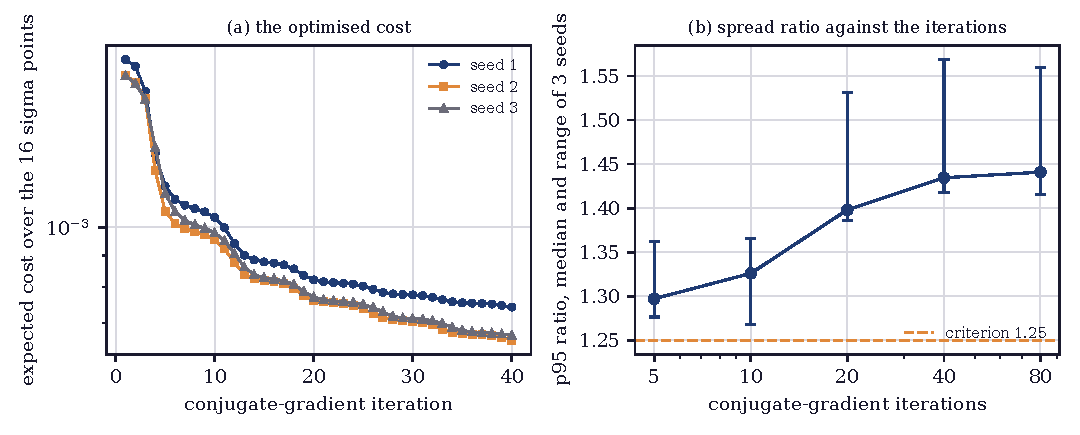
\includegraphics[width=\textwidth]{fig-conv.pdf}
\caption{(a) Expected cost over the 16 sigma points along the 40 conjugate-gradient iterations for seeds 1 to 3 (logarithmic axis). (b) Ratio of the 95th percentiles against the number of iterations, median and range of three seeds, with the criterion of 1.25.}
\label{fig:conv}
\end{figure}
